%TC:macro \cite [option:text,text]
%TC:macro \citep [option:text,text]
%TC:macro \citet [option:text,text]
%TC:envir table 0 1
%TC:envir table* 0 1
%TC:envir tabular [ignore] word
%TC:envir displaymath 0 word
%TC:envir math 0 word
%TC:envir comment 0 0
\documentclass[acmtog]{acmart}
\usepackage{graphicx}
\usepackage{listings}
\usepackage{color}
\usepackage{tikz}

\definecolor{dkgreen}{rgb}{0,0.6,0}
\definecolor{gray}{rgb}{0.5,0.5,0.5}
\definecolor{mauve}{rgb}{0.58,0,0.82}

\lstset{frame=tb,
  language=Java,
  aboveskip=3mm,
  belowskip=3mm,
  showstringspaces=false,
  columns=flexible,
  basicstyle={\small\ttfamily},
  numbers=none,
  numberstyle=\tiny\color{gray},
  keywordstyle=\color{blue},
  commentstyle=\color{dkgreen},
  stringstyle=\color{mauve},
  breaklines=true,
  breakatwhitespace=true,
  tabsize=3
}


\AtBeginDocument{%
  \providecommand\BibTeX{{%
    Bib\TeX}}}


\setcopyright{acmlicensed}
\copyrightyear{2024}
\acmYear{2024}

\citestyle{acmauthoryear}


\begin{document}

\title{Emulating Virtualized ARM TrustZone on a Xen Hypervisor in an x86 Environment}


\author{Yong Li, Linglin Wu, Rui Li}
\authornote{Both authors contributed equally to this research.}
\email{{yonli,linglinwu,ruili}@umass.edu}
\orcid{1234-5678-9012}
\affiliation{%
  \institution{University of Massachusetts, Amherst}
  \city{Amherst}
  \state{MA}
  \country{USA}
}

\renewcommand{\shortauthors}{Yong Li, Linglin Wu, Rui Li}


\begin{abstract} 
  Abstract-The wide adoption of virtualization technologies in embedded systems has brought up the demand for secure environments that protect against privileged adversaries. ARM TrustZone is a hardware-based TEE that provides a basis for securely executing sensitive operations. However, integrating TrustZone with virtualization platforms remains a challenge. In this work, QEMU and Xen are used to establish a robust development environment for emulating ARM TrustZone. QEMU, therefore, enhances TrustZone feature debugging, testing, and verification by offering a platform emulated from ARM for independent work from the actual physical hardware. Xen expands this virtualization capability with this hypervisor, whereby various separated operating systems can execute efficiently and at the same time not compromise on allowing supported TrustZone operations. Taken together, QEMU and Xen are a secure yet versatile combination for exploring and improving the potential of virtual systems' TrustZone. This paper is demonstrating the setup, integration, and evaluation of TrustZone-enabled virtualized environments that provide insights into their performance and practical applications. 
\end{abstract}


    
\maketitle

\section{Introduction}



\subsection{Literature Review}

TEEs combined with virtualization platforms have become increasingly popular over the past years. One such hardware-based TEE is ARM TrustZone, which provides a safe haven for sensitive operations. However, its integration into virtualized systems is still an underexplored area. This section discusses some key contributions in this domain and highlights how our solution stands out.
Li et al. proposed TEEv, a virtualization framework that allows multiple isolated TEE instances to run concurrently on mobile platforms \cite{10.1145/3313808.3313810}. Their architecture, leveraging a hypervisor (TEE-visor), allows for the isolation of TEE instances and reduces security risks related to shared TEEs. However, TEEv focuses mainly on multi-TEE environments and does not discuss the functional integration of ARM TrustZone with hypervisors for system-level virtualization.\cite{7005255} \cite{10.1007/978-3-642-32298-3_1}

Harrison et al. proposed PARTEMU, a modular framework for emulating TrustZone software \cite{247658}. It is based on QEMU and PANDA and allows for the dynamic analysis of real-world TrustZone operating systems and applications. Although very powerful in finding vulnerabilities, PARTEMU does not support the integration of TrustZone with hypervisors like Xen, which plays an important role in virtualized system management.

Yang and Lee used OP-TEE with QEMU to implement TEE Client APIs between the Normal World and Secure World \cite{10.1145/3426020.3426113}. In their work, they have provided a good starting point for security research. Their solution has again been designed for a single-system setup and does not extend the virtualization capability.\cite{10274941} \cite{10.1145/3426020.3426113} \cite{8352425}

Our approach extends these efforts further by incorporating ARM TrustZone into a Xen-based virtualized environment. Unlike TEEv, which focuses on multi-TEE scenarios, our work focuses on taking advantage of TrustZone in order to provide secure services in a single TEE architecture. Finally, QEMU emulates the ARM platforms for ease of debugging, testing, and performance benchmarking. Using QEMU together with Xen in this context provides an extended framework for exploring and enhancing TrustZone's potential in virtualized embedded systems.



\subsection{Motivation}
The growing presence of embedded systems in critical infrastructure has raised the need for better security. On the other hand, hypervisors are powerful yet vulnerable to attacks that might spill over into all systems running on the hardware. This is where ARM TrustZone steps in, providing a TEE that is somewhat isolated from the rest of the system and thus protected against privileged adversaries. Hence, this project will be about studying the possibility of running Xen hypervisor with OP-TEE TrustZone Software support on an ARM QEMU-emulated environment. Through such a study, we will be able to increase the security level of embedded systems by expanding the TrustZone benefits to virtualized environments.



\subsection{Objective}
The key outcome expected is the development of a stable, flexible development environment to try the integration of ARM TrustZone with virtualization technologies. This translates into the following set of concrete objectives:
\begin{itemize}
    \item Port Xen hypervisor featuring OP-TEE (TrustZone Software) running within a QEMU-emulated ARM, to enable emulation of the functionality provided by TrustZone without any dependence on physical hardware.
    \item It will research the performance-security consequences of combining TrustZone and Virtualization: focusing on a probably beneficial trade-off when doing virtualization. Benchmark performance-security using \textit{xtest}, to determine enhancement and security guarantees by TrustZone provided as a result of various methods of deploying the coprocessor in both single and multi-operating system guests.
    \item Basic understanding of how virtualized systems with integrated TrustZone work, which will be helpful in future research and practical applications of embedded systems.
  \end{itemize}

 This work not only addresses current hypervisor-TrustZone integration limitations but also provides the foundation to advance both security and functionality for virtualized embedded systems.



\section{Background}

\subsection{ARM TrustZone Technology}


ARM TrustZone is a hardware-based security technology integrated into many ARM processors, widely used in mobile devices and embedded systems. It provides a strict separation between two execution environments: the Secure World and the Normal World \cite{10.1145/3426020.3426113, partemu,10.1007/978-3-030-22496-7_9}.

The Secure World allows a TEE for sensitive operations to be executed safely, without the possibility of any threat from the Normal World. The most important uses of the Secure World are as follows:

\begin{itemize}
  \item Storing cryptographic keys securely.
  \item Processing financial transactions and payments.
  \item Running secure boot mechanisms to validate system integrity.
\end{itemize}\cite{ 10.1145/3313808.3313810, partemu,10.1007/978-3-030-22496-7_9}.

The basic principle behind the TrustZone design is being an isolated world from non-trust parts, providing the means to enhance embedded and mobile system security.

\subsection{Comparison of Hypervisor Architectures}
 
\begin{figure}[ht]
  \centering
  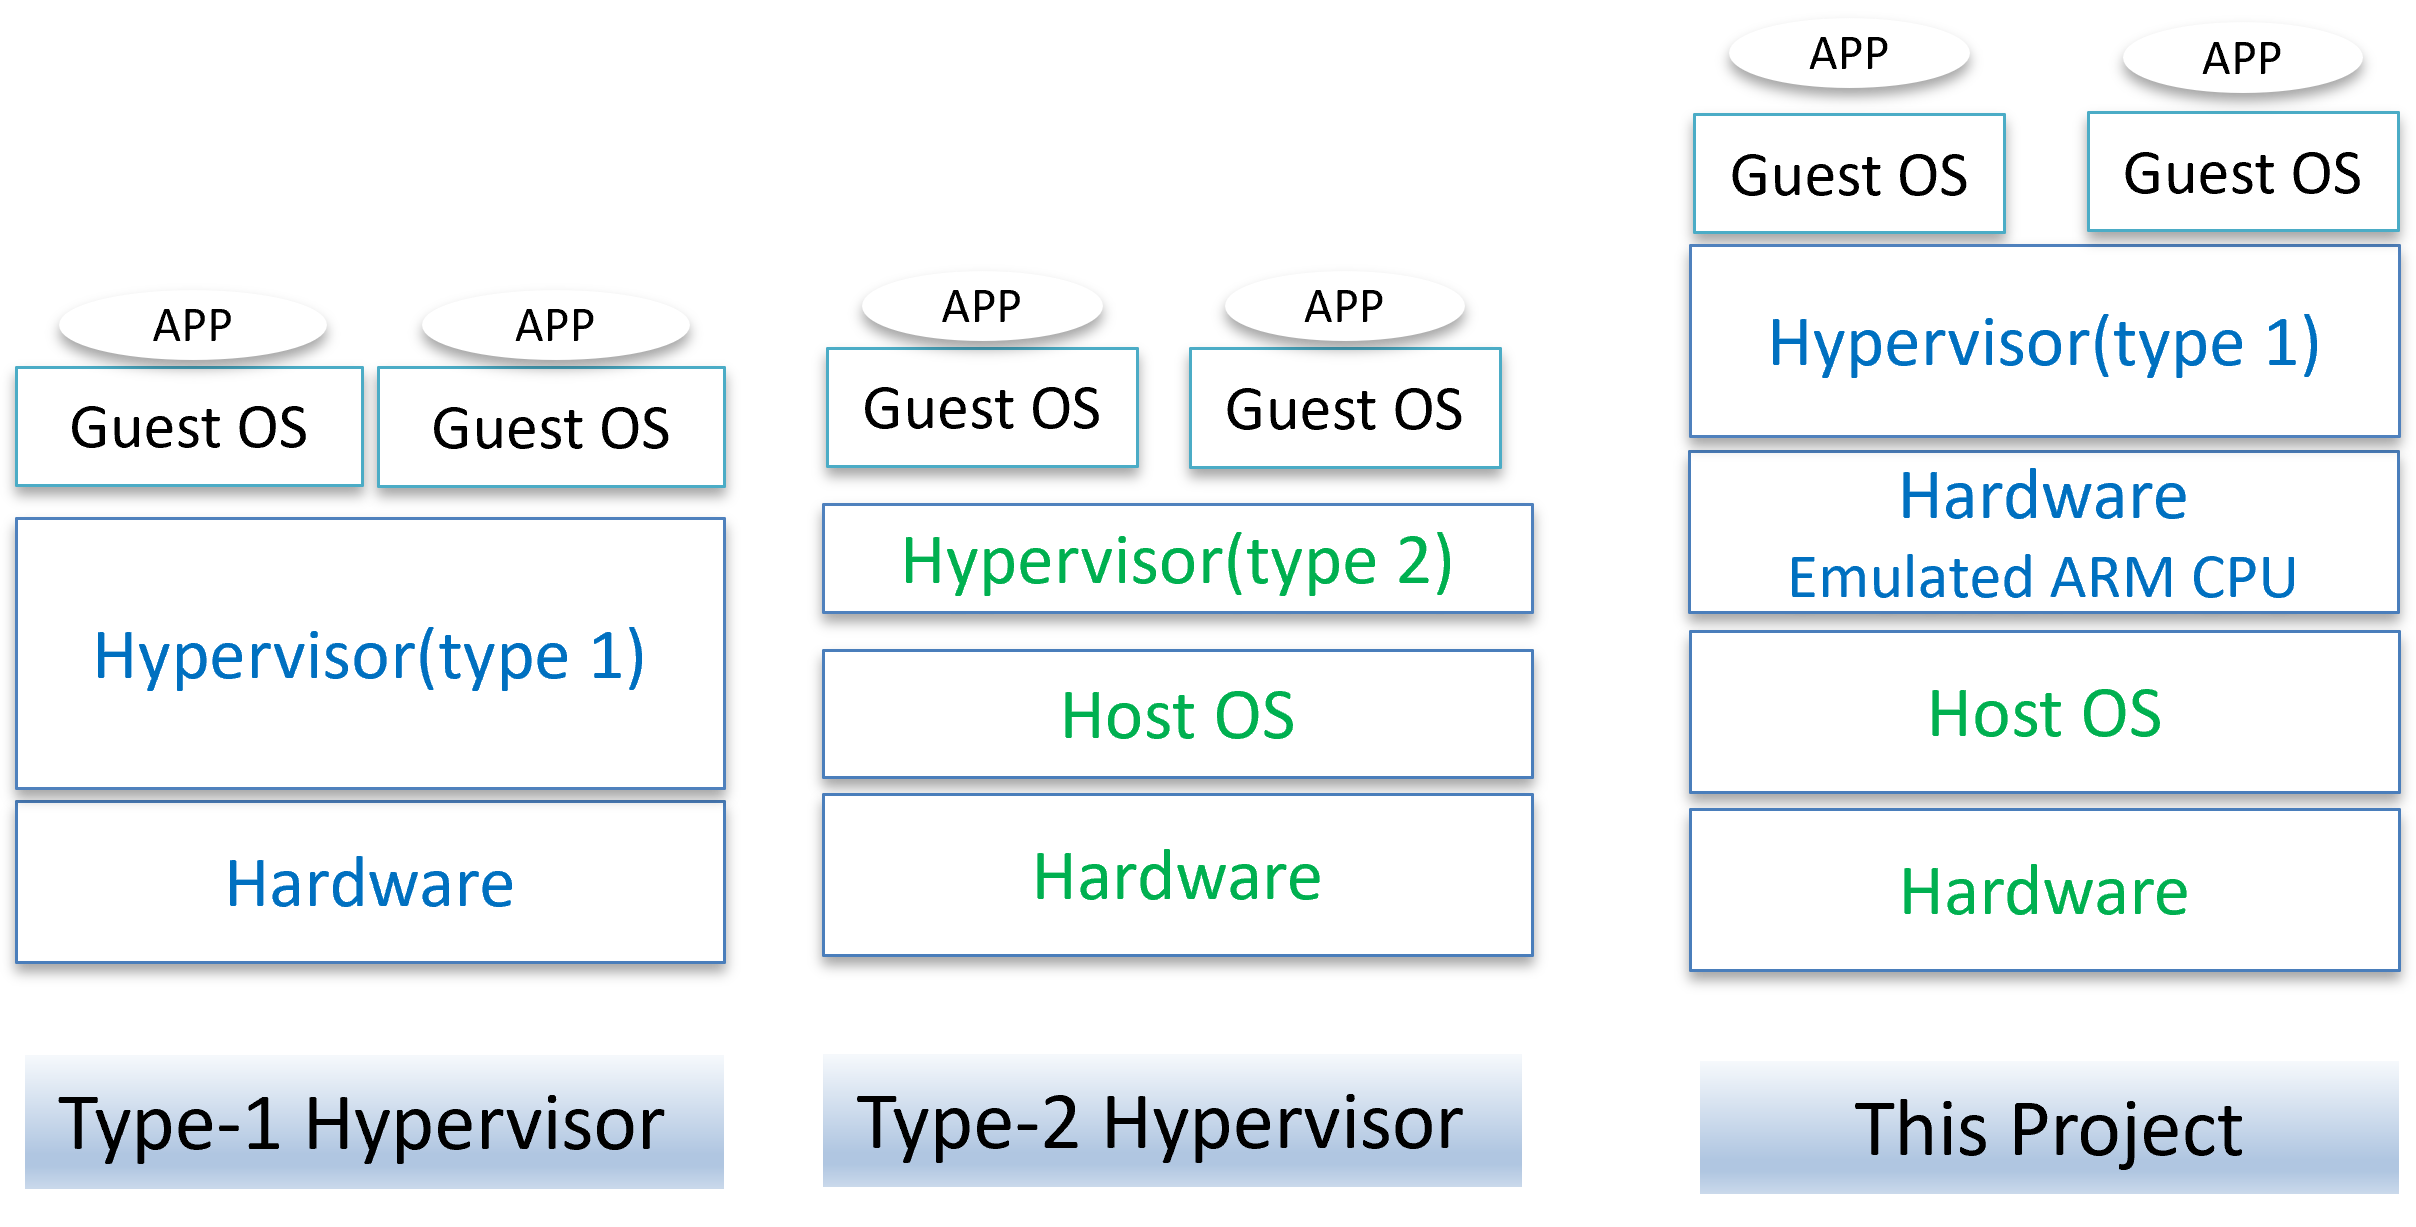
\includegraphics[width=\columnwidth]{images/type12_hyper.png}
  \caption{Type1, Type2 and this Project used Hypervisor}
  \label{fig:compare_hypervisor}
\end{figure}


Figure~\ref{fig:compare_hypervisor} highlights the hypervisor architectures of Type-1 and Type-2 hypervisors compared to the structure used in this project. The hypervisor set-up in this project is very different from the conventional Type-1 and Type-2 hypervisors, considering both complexity and flexibility.

\paragraph{Type-1 Hypervisor:}
A Type-1 hypervisor is also known as a bare-metal hypervisor. It runs directly on the underlying hardware. The hypervisor and its guest operating systems have exactly the same architecture as the hardware, for example, x86 or ARM. Such a design provides high performance and direct hardware access. However, it relies fully on the hardware platform.

\paragraph{Type-2 Hypervisor:}
A Type-2 hypervisor, on the other hand, executes on top of a host operating system and depends on this host OS to manage hardware resources. Similar to Type-1 hypervisors, it also requires that both the hypervisor and guest OSes use the same architecture as the base hardware. This is easier to set up but has more overhead and is tightly coupled to the hardware platform.


\paragraph{This Project's Hypervisor Architecture:}
On the other hand, this project has adopted the hypervisor architecture, which decouples the hypervisor and guest operating systems from the original hardware architecture. Using QEMU, an emulation of the ARM CPU is allowed, thereby allowing the Xen Type-1 hypervisor and guest OSs (ARM architecture) to run on an x86 host machine. This design in a hardware-independent way avoids the architectural limitation of traditional Type-1 and Type-2 hypervisors, allowing cross-platform testing and development.


\paragraph{Advantages of This Project's Architecture:}
The added complexity of this setup is justified by the increased flexibility it provides:

\begin{itemize}
    \item \textbf{Cross-Platform Compatibility:} This allows the hypervisor and guest OSes to execute on any hardware, completely independent of the actual architecture, by emulating the ARM CPU.
    \item \textbf{Hardware Independence:} Unlike traditional hypervisors, the virtualization stack is not bound to native hardware architecture, which allows flexibility in secure experimentation, especially when physical ARM hardware is not available.
    \item \textbf{Enhanced Testing and Development:} This architecture is ideal to develop and test secure applications that leverage TrustZone since it provides a controlled, reproducible virtualized environment.
\end{itemize}
This project will be able to show that QEMU, Xen, and OP-TEE together can form a highly versatile and secure virtualization stack, breaking the limits of traditional hypervisor architectures.


\subsection{QEMU: A System Emulator}
QEMU is a multi-purpose system emulator that is widely used in research and development to emulate many architectures, including x86, ARM, MIPS, RISC-V, and more. It is one of the enabling factors for cross-platform development and testing without requiring physical hardware \cite{efficient_virtualization, partemu, qemu_fast_portable}. \cite{10.5555/1247360.1247401}

QEMU plays an important role in this project because it provides an ARM-emulated environment into which ARM TrustZone can be combined with the Xen hypervisor. This is because it emulates a full system: it emulates CPUs, devices, kernels, and applications - and is ideal for the evaluation process of TEEs like OP-TEE. The QEMU system would provide complete emulation of a computer system, including peripherals, thereby allowing numerous virtual machines to be run virtually on one physical host \cite{efficient_virtualization}.

QEMU operates in various modes:


\begin{itemize}
    \item \textbf{User-mode emulation:} This mode enables QEMU to run single Linux or Darwin/macOS programs compiled for other instruction sets. It will translate system calls for endianness and architecture compatibility, but it does so quite well and is convenient for cross-compilation and cross-debugging.
    \item \textbf{System emulation:} In full-system emulation mode, QEMU emulates a complete computer with its devices. This feature makes it possible to run several guest operating systems, including Linux, Windows, Solaris, and BSD, on various architectures, including ARMv7, ARMv8, x86, among others \cite{qemu_fast_portable}.
    \item \textbf{Hypervisor support:} QEMU can be used either as a VMM or as a device emulation back-end for virtual machines running under a hypervisor. Combined with KVM or hypervisors such as Xen, near-native execution speeds are achieved while still offering broad emulation capabilities \cite{partemu}.
\end{itemize}


One of the central features of QEMU is the use of Tiny Code Generator to dynamically translate guest CPU instructions into their equivalent host assembly instructions. This flexibility and efficiency in running virtualized workloads are especially important in developing and benchmarking systems that include ARM TrustZone.

QEMU provides the base for this project, exploring secure and virtualized environments with ARM TrustZone through its powerful emulation features and support for a wide variety of architectures and virtualization setups.


\section{System Design: Introduction to the Virtualization Stack}

This section covers the design and implementation of a virtualized environment that can enable QEMU-based TrustZone applications. We will explain how to enable a TrustZone-based application running in a virtualized environment on QEMU on an X86 CPU. That will be done by incrementally adding virtualization technologies to an already existing base ARM CPU with TrustZone. This introduces the hypervisor, which is used to virtualize the TEE rich OS and to virtualize the ARM CPU with QEMU. Following is a high-level view of the stack:

\begin{itemize}
    \item TrustZone Application (via OP-TEE)
    \item Linux Guest OS
    \item Hypervisor (Xen)
    \item QEMU (emulates ARM CPU)
    \item AnyCPU (host OS)
\end{itemize}

We will explore each step in detail, showing how the system is built up layer by layer.

\subsection{Step 1: Bare Metal Machine. OS directly running on ARM CPU}

First, it shows the simple configuration where the Linux OS runs on an ARM-supported CPU by TrustZone. This TrustZone provides a hardware-based isolation mechanism which divides the CPU into two "worlds": the secure world - that is, TrustZone - and the non-secure world, Linux. Here, one can see that Linux is directly communicating with the ARM CPU, running in a non-secure world, whereas applications run in the secure world. This is the most simple form of running Linux with support for TrustZone.
\begin{figure}[ht]
  \centering
  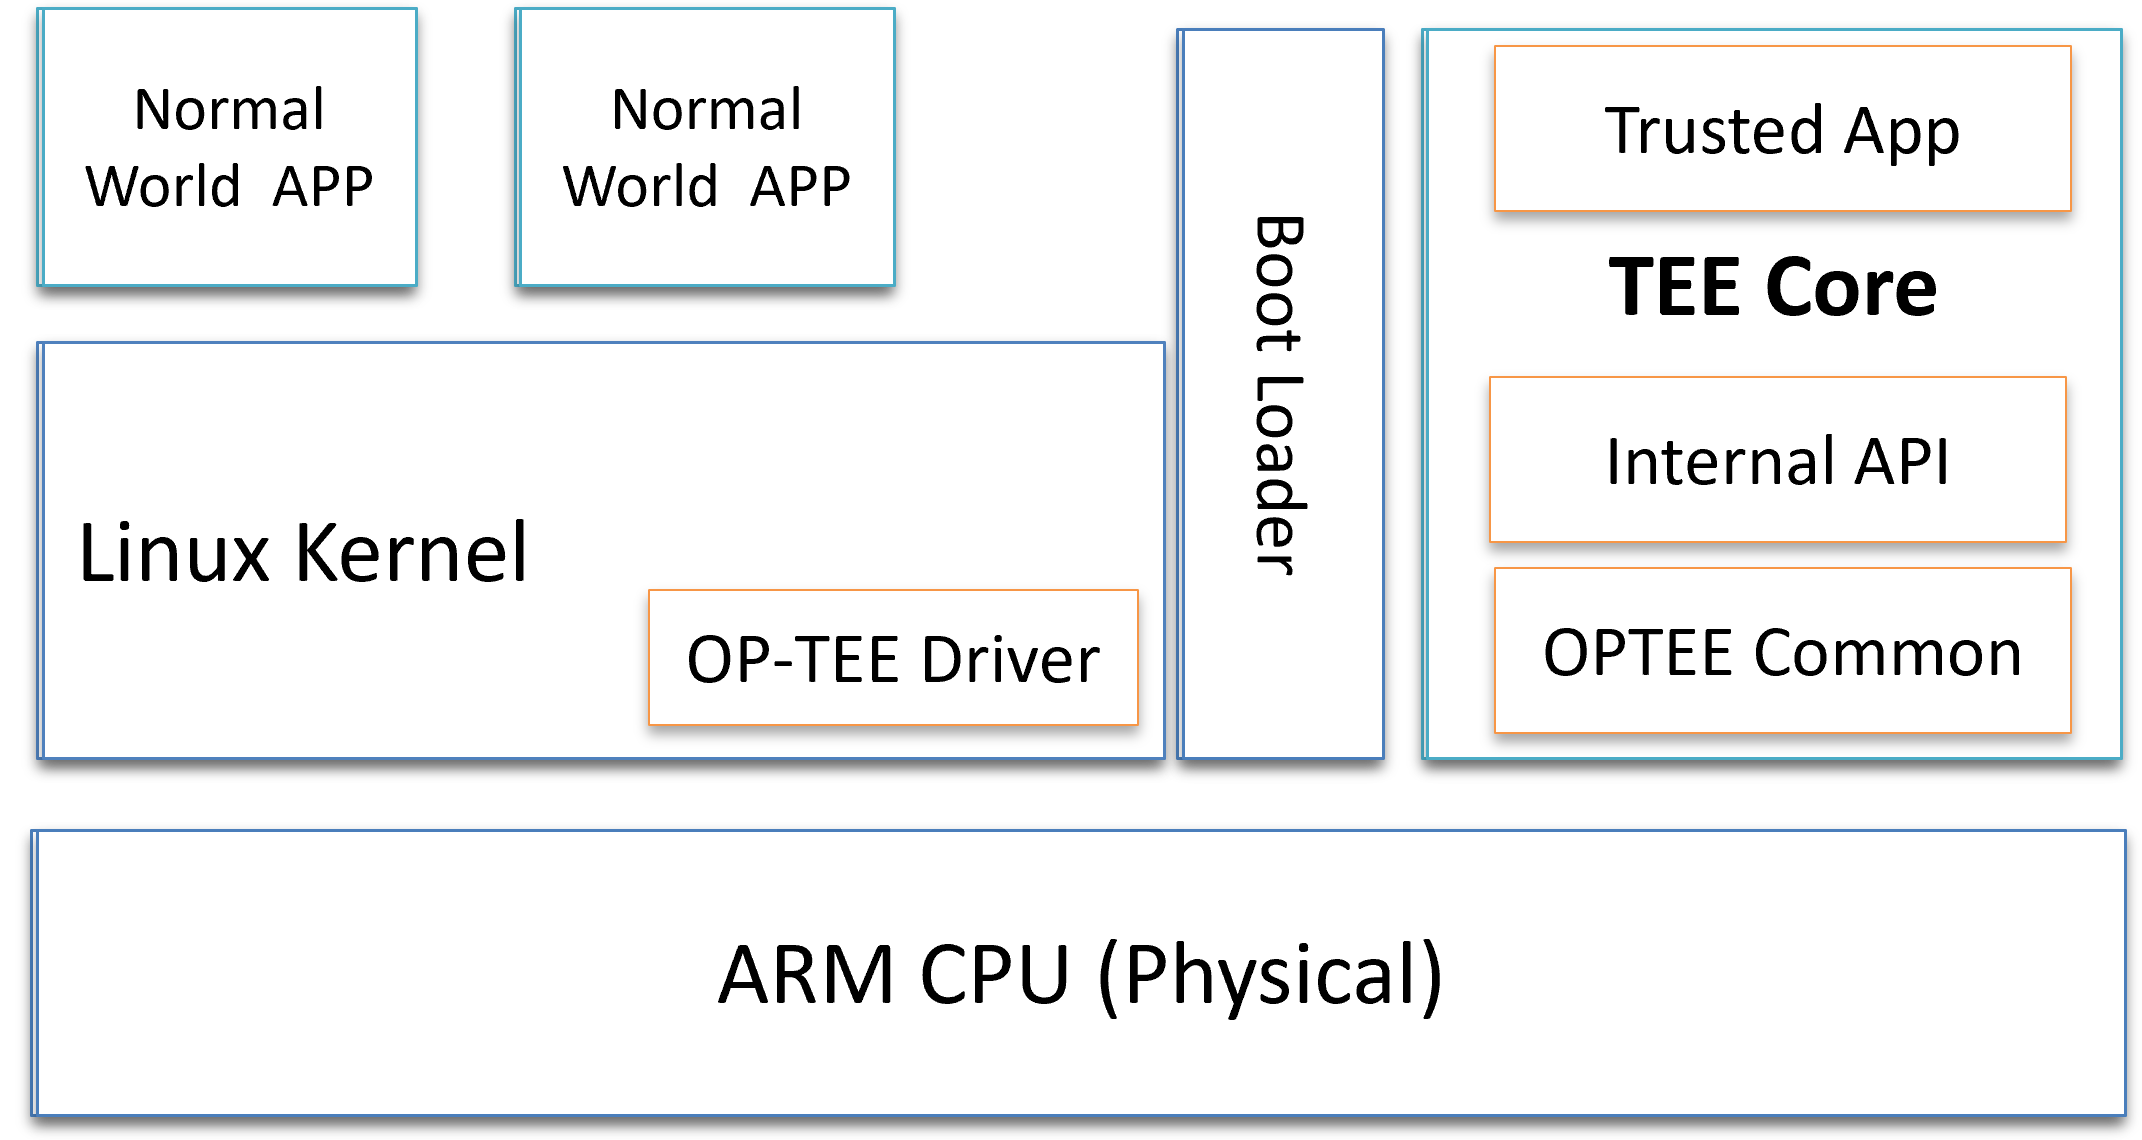
\includegraphics[width=\columnwidth]{images/1.png}
  \caption{ARM Trusted App, no virtualization}
  \label{fig:image_label}
\end{figure}



\subsection{Step 2: Virtualize the OS by introducing Hypervisor}
This introduces the system to the hypervisor: Xen. A hypervisor-also called a VMM-further abstracts the hardware, thus offering the running of multiple OSs on one computer. So, Xen is going to run on top of the ARM CPU and then virtualize Linux, itself an OS, running as a guest OS. A hypervisor makes the operating systems-even guest ones-much farther away from the hardware so no guest OS acts upon it directly. This will provide the possibility to execute the secure TrustZone application along with the virtualized Linux OS.

This is a very important step that involves introducing the hypervisor in order to enable virtualization of the system. In this case, the hypervisor used, Xen, executes directly on the ARM CPU and it sits between the hardware and the OSes to run atop of it.

In our setup, a Type 1 hypervisor is used, namely Xen. Xen runs directly on the ARM hardware; this allows it to manage most of the physical resources of the system and give them - as efficiently as possible - to VMs. The presence of Xen introduces the concept of domains:

\begin{itemize}
    \item \textbf{Domain 0 (Dom0):} This is the privileged domain, which directly accesses hardware resources and controls other domains. It typically runs a Linux-based OS, which performs the tasks of managing virtual devices and, in general, the virtualization environment.
    \item \textbf{Domain U (DomU):} These are the unprivileged domains or virtual machines running on top of Dom0. Each DomU will run its own guest operating system, which in our case is a Linux OS. The DomU does not have direct access to hardware, and interactions with the hardware must go through Dom0 or the hypervisor.
\end{itemize}

Xen ensures that these domains remain separated from each other in order not to let the problems occurring in one domain compromise any other. That is because the isolation principle is key for virtualization, meaning running multiple guest OSes securely on the same hardware without disturbing the others.



\begin{figure}[ht]
  \centering
  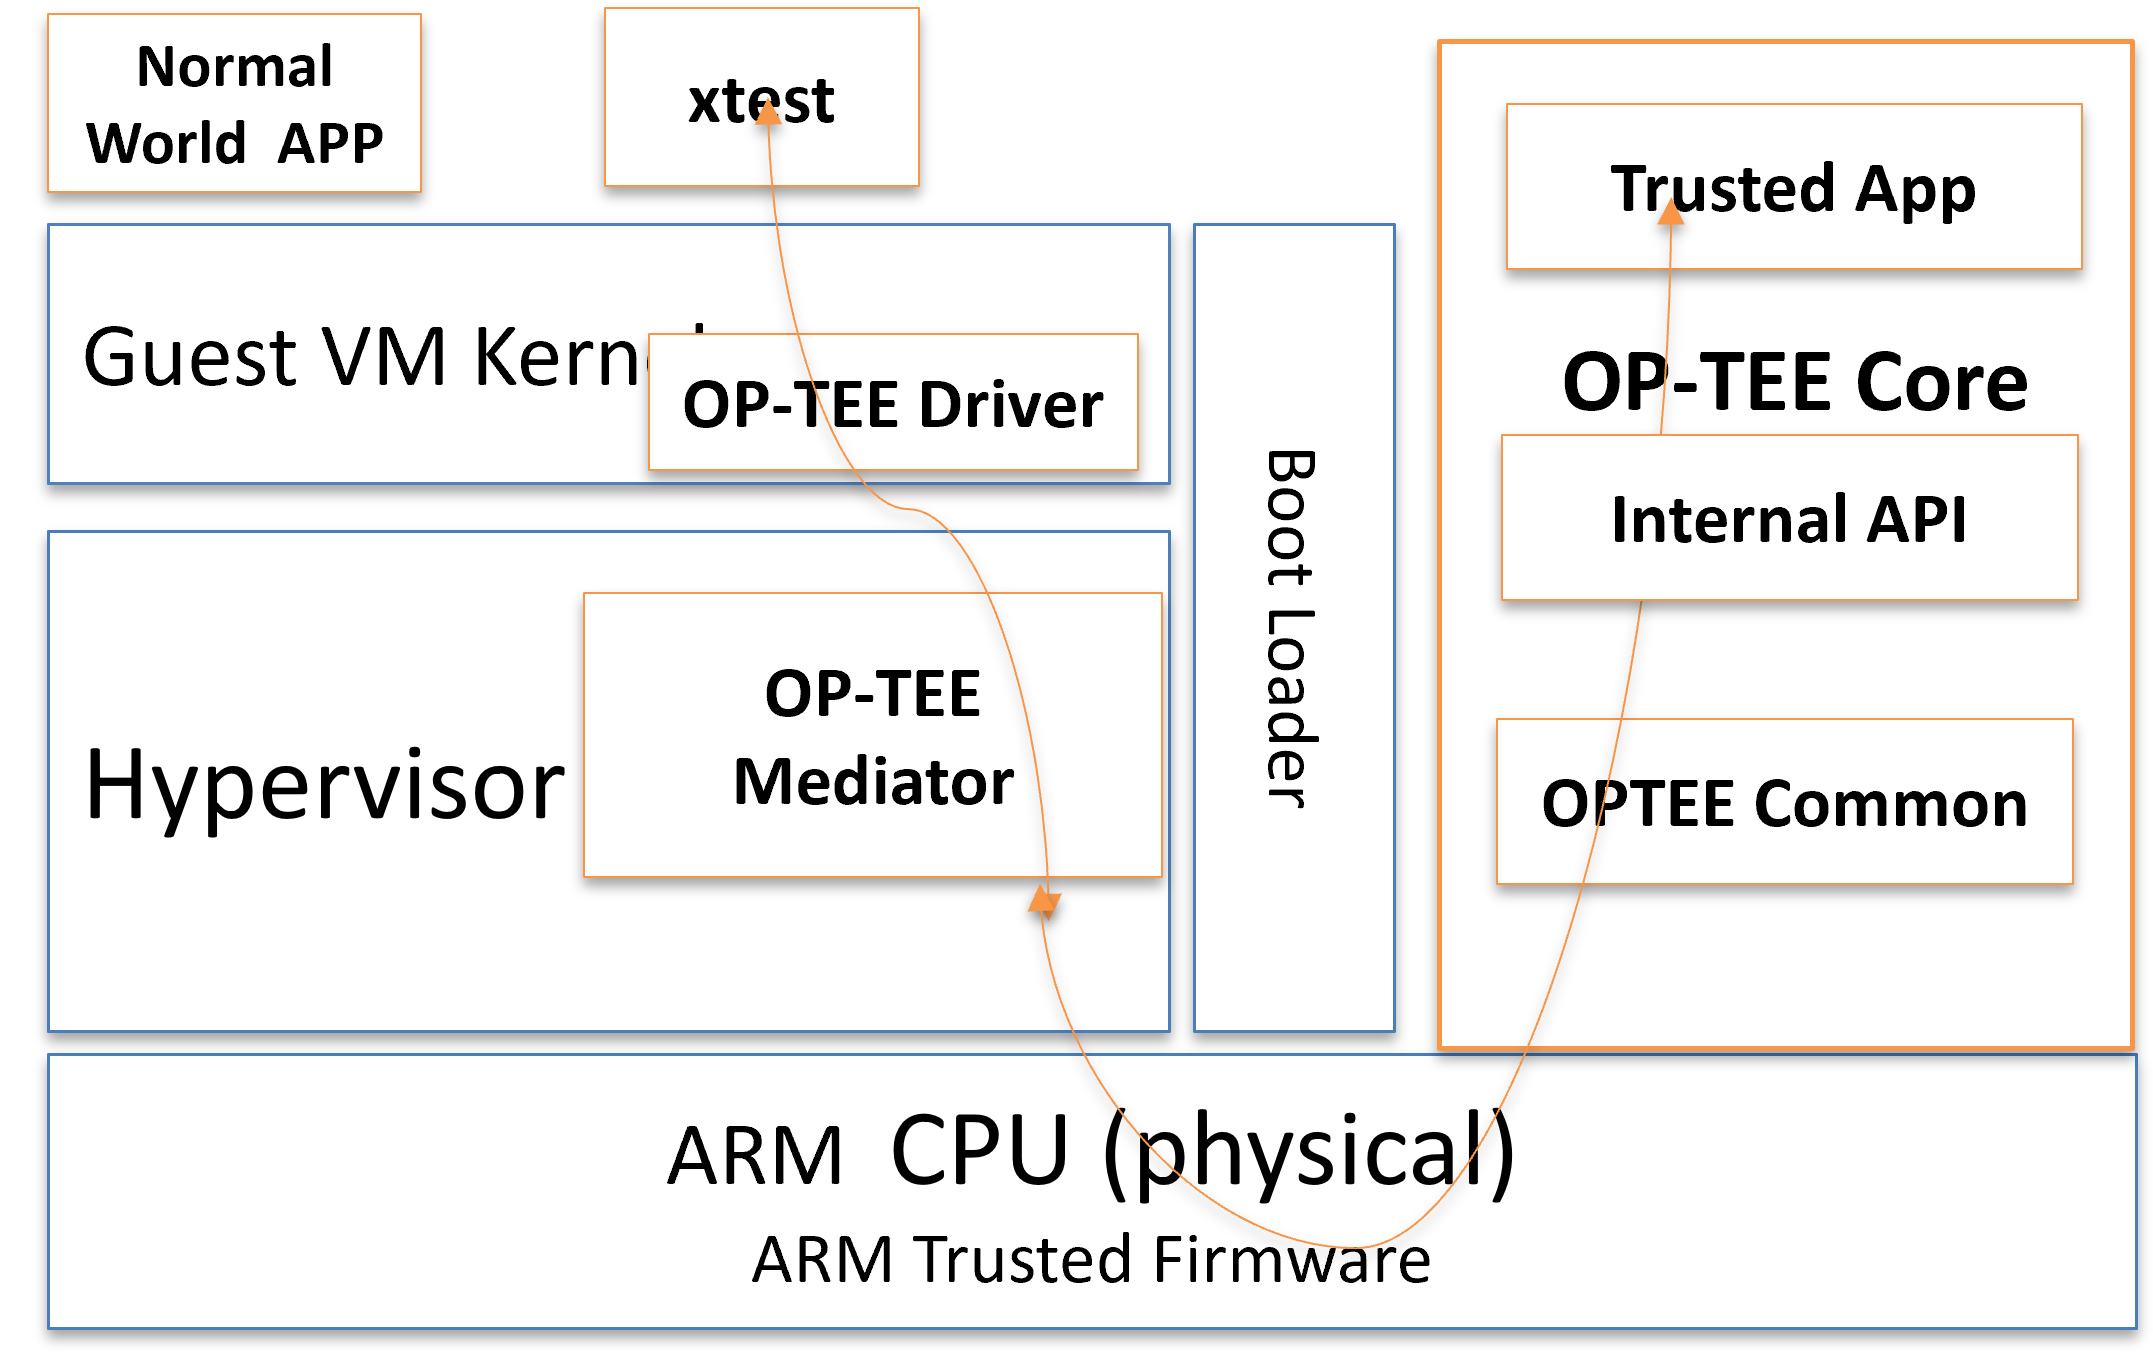
\includegraphics[width=\columnwidth]{images/2.png}
  \caption{Linux OS is virtualized by Xen hypervisor}
  \label{fig:image_label}
\end{figure}


\subsection{Step 3: Virtualizing the ARM CPU by QEMU}

The last level of the virtualization stack is using QEMU to emulate the ARM CPU on a non-ARM host machine, like an x86-based one. QEMU will offer complete system emulation, allowing the ARM architecture to be self-sufficient with no use of physical hardware. Such a configuration would mean the Xen hypervisor can run on top of the virtualized ARM CPU, which again will manage guest operating systems and also provide functionality related to TrustZone.

In this configuration:
\begin{itemize}
    \item \textbf{TrustZone Application:}  TrustZone application runs securely inside ARM TrustZone, separated from the non-secure world.
    \item \textbf{Linux Guest OS:} runs in the non-secure world on top of the virtualized ARM hardware.
    \item \textbf{Hypervisor (Xen):} to provide virtualization layer, maintain resource isolation and security.
    \item \textbf{QEMU (ARM CPU Emulator):} Provides emulation for the ARM architecture, allowing the stack to run on a non-ARM host.
    \item \textbf{Host OS (AnyCPU):} Provides the physical resources for Virtualization and Emulation.
\end{itemize}

\begin{figure}[ht]
  \centering
  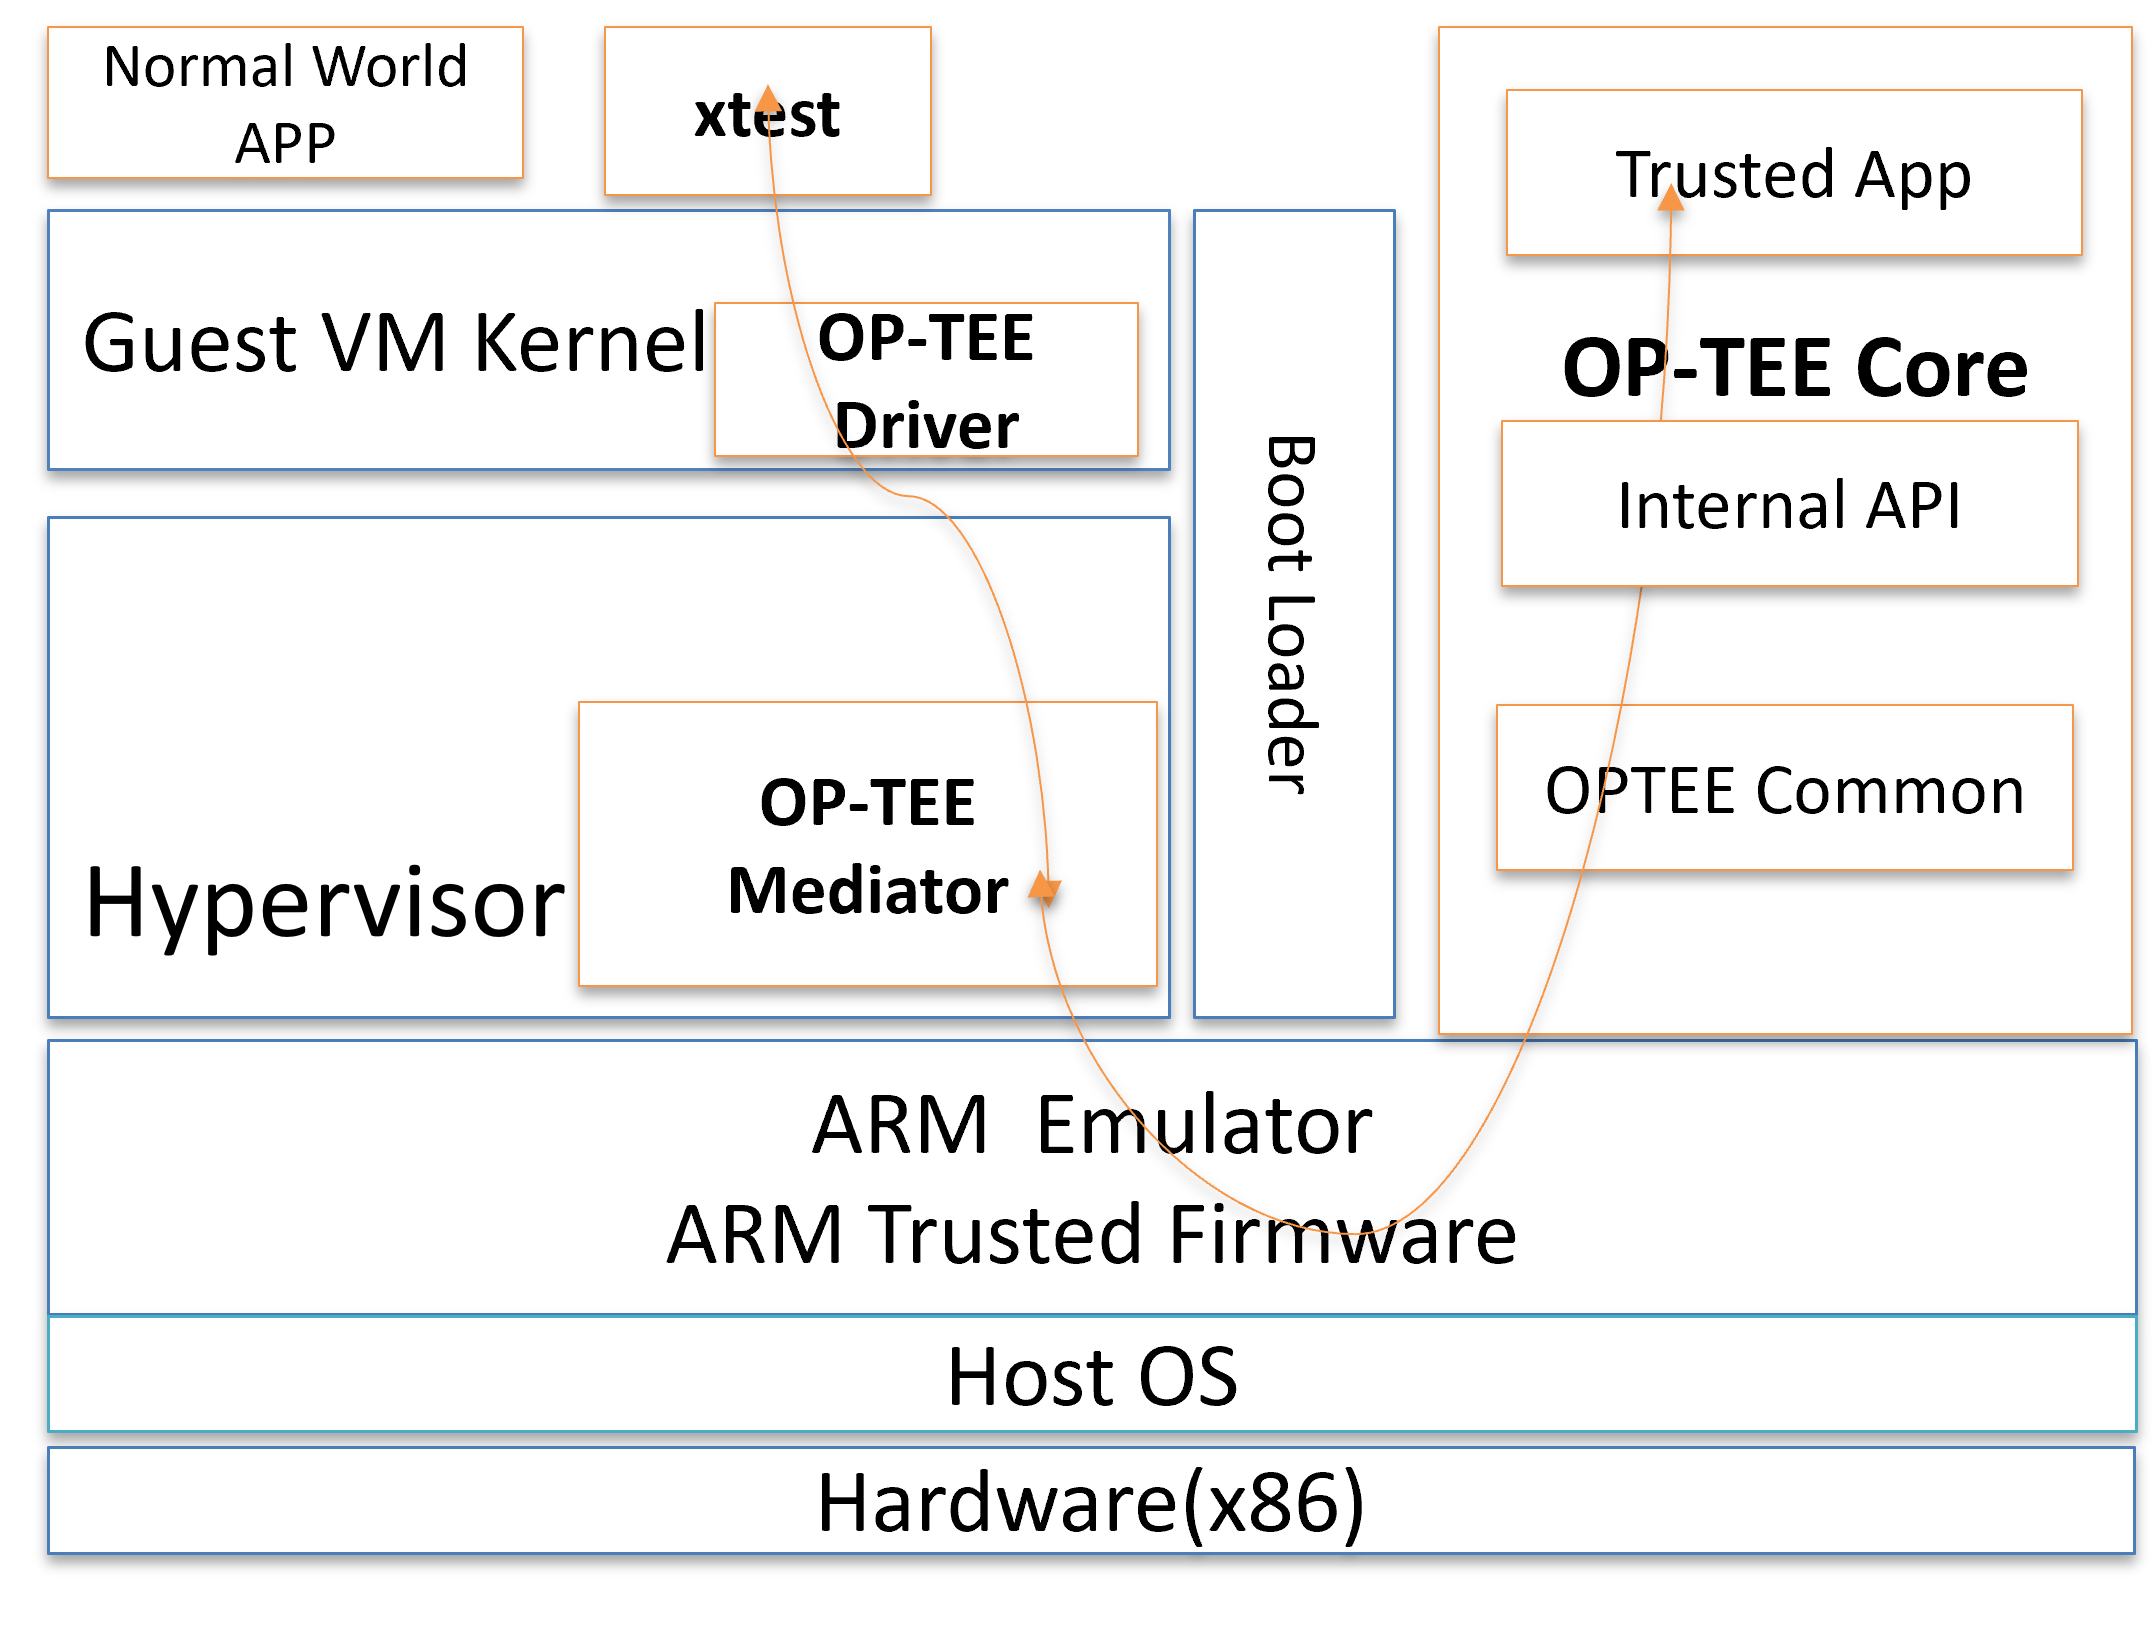
\includegraphics[width=\columnwidth]{images/3.png}
  \caption{Final Virtualization Stack. ARM Processor is virtualized by QEMU}
  \label{fig:virtual_stack}
\end{figure}

\subsection{Recap}
The basic thought in designing the virtualization stack has been incremental towards the enabling of TrustZone applications, which are flexible but secure.

\begin{itemize}
    \item \textbf{Step 1: Bare-Metal Setup:} It was also installed to run directly on an ARM CPU with TrustZone support, which provides the basic hardware-based isolation between Secure World and Non-Secure World.
    \item \textbf{Step 2: Virtualization with Xen:} The Xen hypervisor virtualized the ARM CPU, which can support multiple independent guest operating systems running simultaneously.
    \item \textbf{Step 3: Emulation with QEMU:} QEMU was used to emulate the ARM CPU, which allowed the entire stack to run without issue on non-ARM hardware, such as that using x86-based platforms.
\end{itemize}

This will be demonstrated in an integrated step-by-step approach with virtualization and emulation technologies to show a scalable framework for testing, debugging, and researching secure applications in virtualized embedded systems. Combining strengths from QEMU and Xen, this stack reaches hardware independence with robust isolation, thereby making it a versatile tool to advance TrustZone-based research.




\section{Implementation}
This section describes the implementation of the virtualization stack to allow TrustZone-based applications.

Most of the virtualization stack was implemented based on the work of Denis Obrezkov, which gave guidelines on how to set up Xen, QEMU, and Linux configurations \cite{obrezkov2019xen}. Nevertheless, our work is using the latest versions of the software in order to be compatible and have better functionality. In terms of TEE parts, we used the official OP-TEE documentation on how to correctly implement and configure secure world operations \cite{optee_docs}.


\subsection{System Components}
Our system uses the following key components to perform the tasks assigned to it: 
\begin{itemize}
  \item \textbf{Trusted Execution Environment:} Trusted Application running in the Normal World and OP-TEE Core.
    \item \textbf{Hypervisor:} Xen hypervisor, experimental OP-TEE support, providing strong virtualization competency.
    \item \textbf{ARM Emulator:} QEMU to emulate the ARM CPU and enable the virtualization stack on x86-based hardware.
    \item \textbf{Guest Operating Systems:} Linux kernel, compiled for both secure and non-secure environments, running as guest OSes.
    \item \textbf{Bootloader:} U-Boot for system initialization and loading of the Xen hypervisor and guest operating systems.
    \item \textbf{Utility Tools:} BusyBox to create a lightweight root filesystem for the guest Linux environments.
\end{itemize}


The key software components used in our implementation include: 

\begin{itemize}
  \item \textbf{OP-TEE:} Version 4.3.0

  \item \textbf{Xen:} Version 4.18.3
  \item \textbf{QEMU:} Version 9.1.0

    \item \textbf{BusyBox:} Version 1.37.0
    \item \textbf{Linux Kernel:} Version 6.1.18

    \item \textbf{U-Boot:} Version 2024.07


\end{itemize}



\subsection{Role of the Hypervisor in OP-TEE Integration}
This is to allow the hypervisor to manage safe interactions between the guest virtual machines and OP-TEE. Different challenges exist for virtualization and security on OP-TEE being directly called by the virtual machines, such as virtual address address space, requiring OP-TEE to be cognisant of VM creation/ destruction and which VM the calling is coming from. Besides, the hypervisor also provides memory isolation such that a VM cannot reference another VM's memory when operating against OP-TEE. The hypervisor solves these challenges to securely and efficiently integrate OP-TEE in the virtualized environment. OP-TEE needs to track the life cycle of VMs. So it provides two special
calls:

\begin{itemize}
  \item \texttt{OPTEE\_SMC\_VM\_CREATED VMID}
  \item \texttt{OPTEE\_SMC\_VM\_DESTROYED VMID}
\end{itemize}

Hypervisor notifies OP-TEE for VM creation or destruction by issuing the above SMCs.


\subsection{OP-TEE Virtualization Support: XEN TEE Mediator}
OP-TEE has experimental support for virtualization, enabling one OP-TEE instance to securely run TAs originating from several VMs. It does this by keeping the states of the different VMs isolated within OP-TEE so that operations coming from one VM cannot affect another. Such isolation is crucial for the integrity and security of TEEs in virtualized systems.
In a virtualized environment, OP-TEE relies on the hypervisor to mediate access between VMs and the TEE. The hypervisor does the following:

\begin{itemize}
  \item Identifying which VM is making a request to OP-TEE.
  \item Informing OP-TEE about the creation and destruction of VMs to manage secure resources effectively.
  \item Translating Intermediate Physical Addresses (IPAs) used by VMs into Physical Addresses (PAs) required by OP-TEE, as OP-TEE cannot process IPAs directly.
\end{itemize}
It achieves this through a dedicated Xen component known as "TEE Mediator." This acts to securely relay information from the VM to OPTEE and vice-versa while ensuring proper isolation and performing proper address translations in both ways.

Basic support for OP-TEE within Xen can be enabled through an interactive, menu-based configuration, or as a noninteractive, command-line configuration.


\paragraph{Interactive Menu Configuration:}
\begin{enumerate}
    \item Navigate to the Xen source directory.
    \item Run the \texttt{make menuconfig} command to access the Xen configuration menu.
    \item Enable the \texttt{OPTEE} option under the "Architecture Features" section.
    \item Ensure that the "TEE mediators" option is also enabled.
    \item Save the configuration and exit the menuconfig tool.
    \item Compile and install Xen with the updated configuration.
\end{enumerate}

The specific path in the Xen interactive menu for enabling OP-TEE support is:
\texttt{Xen/arm 4.18.3 configuration -> Architecture Features -> TEE mediators -> Enable OP-TEE mediator (UNSUPPORTED)}.

\paragraph{Non-Interactive Command-Line Configuration:}
Alternatively, the configuration can be performed directly by modifying the Xen `.config` file. The following changes enable OP-TEE support: edit the \texttt{xen/.config} file and update the following options:

\begin{lstlisting}[language=make, caption=Enable OP-TEE Support in Xen Configuration]
# Xen configuration file: xen-4.18.3/xenxen/.config

CONFIG_TEE=y       # Enable Trusted Execution Environment (TEE) support
CONFIG_OPTEE=y     # Enable OP-TEE mediator support
\end{lstlisting}


Either way, the enabling of OP-TEE support allows Xen to securely manage interactions between VMs and the Trusted Execution Environment. It becomes crucial for testing and deploying TrustZone-based applications on virtualized environments.


\subsection{OP-TEE Linux Kernel Support}
The OP-TEE driver in the guest VM kernel is essential for the guest OS to interact securely with the TEE provided by OP-TEE. In a virtualized environment, the hypervisor manages hardware resources on behalf of guest VMs, but direct access to the features of TrustZone is not inherently provided to such VMs. The OP-TEE driver acts as an intermediary to the requests of guest applications for secure processing to OP-TEE. In this way, it ensures that all security-sensitive operations-such as cryptographic computations and key storage-are executed in the TEE without disclosure of sensitive data to an untrusted hypervisor or other guest VMs. Furthermore, the driver abstracts the complexity of managing TrustZone interactions, allowing for smooth use of the OP-TEE services from within the virtualized environment, thereby increasing the security features of the guest VM.

To enable the OP-TEE driver in the guest VM kernel, configuration should be made inside the Linux kernel menuconfig tool. The path to reach this driver in order to configure it is:

\texttt{.config - Linux/x86 6.1.18 Kernel Configuration -> Device Drivers -> Trusted Execution Environment Support}

The following commands and configurations are applied via the command line:
\begin{lstlisting}[language=make, caption=Enabling OP-TEE in the Linux Kernel Configuration]
 
  # Linux configuration file: linux-6.1.18/.config
      CONFIG_XEN=y          # Enable Linux Kernel support for XEN
      CONFIG_XEN_DOM0=y     # Support Linux running as a Xen Dom0 guest

      
      CONFIG_TEE=y          # Enable Linux Kernel support for Trusted Execution Environment (TEE) 
      CONFIG_OPTEE=y        # Enable Linux Kernel support for OP-TEE
\end{lstlisting}


\section{Benchmark Performance Analysis}

The \textit{xtest} A benchmark suite was run in order to evaluate the performance of the OP-TEE TEE in the context of our virtualization stack. These results are important in understanding the feasibility of using OP-TEE with Xen and QEMU for enabling secure applications in virtualized embedded systems.

\subsection{Results Overview}
The benchmark suite ran successfully through the 24 sub-tests with no failures; in summary, the virtualized set up OP-TEE environment had shown stability. Key observations:

\begin{itemize}
    \item \textbf{Trusted Storage Performance:} Writes performed well for smaller sizes-28.57 kB/s for 1 KB, but it tumbled to 17.09 kB/s in the case of big sizes such as 1 MB. Read operations are always better than writes with maximum of 250 KBs when 2 KB can fit inside cache and for 1MB dropped down to 134.95 kB/s.
    \item \textbf{Cryptographic Performance:} 
    \begin{itemize}
        \item SHA1 averaged 0.48 MiB/s, while SHA256 was much faster at 2.22 MiB/s, showing the efficiency of the TEE in performing secure hash operations.
        \item AES-ENCRYPTION was quite stable; for example, ECB mode had 0.61 MiB/s, while CBC mode had 0.63 MiB/s.
    \end{itemize}
    \item \textbf{Rewriting Data:} Rewrite also followed a similar pattern to write: for smaller sizes, it was quite efficient but bigger file sets sharply lowered the speed.
\end{itemize}

\subsection{Project-Specific Insights}
The results are very close to the objectives of this project, which means it is feasible to integrate OP-TEE with a Xen-based virtualized environment on QEMU. Key takeaways include:

\begin{itemize}
    \item \textbf{Secure Storage Limitations:} While the TEE securely protects storage operations, performance degradation with respect to larger data sizes does bring out potential bottlenecks for high-throughput applications. This falls in line with testing the limitations within the current implementation, which was the focus of the project.
    \item \textbf{Cryptographic Workloads:} Such a high score in SHA and AES benchmarks again proved OPTEE to be suitable for performing cryptographic tasks in the secure environment, which is crucial for this project focused on studying whether the TEE would be able to support security-critical applications in virtualized setups.
    \item \textbf{Single-VM Context:} Benchmarks indeed confirm that in the current configuration of a single VM, OP-TEE is functionally stable, but the project requirement to support multiple VMs complicates things since performance implications for multi-VM setups remain unexplored.
\end{itemize}

\subsection{Implications for Virtualized Embedded Systems}
Results will highlight the strengths and challenges of using OP-TEE in virtualized environments.
\begin{itemize}
    \item \textbf{Strengths:} Efficient handling of cryptographic operations, secure isolation was in place, meaning that OPTEE may achieve appropriate security services within a virtualized system.
    \item \textbf{Challenges:} Performance degradation in case of large-scale storage operations, support for multiple VMs are the key areas that need refinement before going into production-level demands.
\end{itemize}

Overall, the benchmarks show that the integration of OP-TEE with Xen and QEMU offers a secure and functional foundation for virtualized embedded systems. Future work will focus on addressing identified limitations to scale this solution for multi-VM environments, aligning with the project's long-term objectives.



\section{Challenges}
The implementation of the virtualization stack encountered several problems. Some problems were indeed real mistakes in the original tutorial \cite{obrezkov2019xen}, while others involved differences introduced by software updates, as we used significantly newer versions of Xen, QEMU, Linux, U-Boot, and OP-TEE. That is, five years passing by means lots of changes in behavior, configuration options, compatibility requirements, which require readjustments and debugging to match the updated software ecosystem.



\subsection{BusyBox Hardware Acceleration Compatibility}
That is, for example, to compile BusyBox to run on QEMU with Xen, all HWA should be turned off. Most virtualized environments don't support direct hardware acceleration, like NEON on ARM platforms. Because of this, enabling HWAs at compile time may result in build breaks or runtime problems because emulated environments don't support hardware-accelerated instructions.

Due to compatibility reasons, HWA should be explicitly disabled in BusyBox configuration to make the build consistent with the constraints of the virtualized environment.

To compile BusyBox without hardware acceleration:

\begin{lstlisting}[language=bash, caption=Solution to HWA Fault]
# Disable Hardware Acceleration in configuration
sed -i 's/CONFIG_SHA1_HWACCEL=y/CONFIG_SHA1_HWACCEL=n/' .config
sed -i 's/CONFIG_SHA256_HWACCEL=y/CONFIG_SHA256_HWACCEL=n/' .config
\end{lstlisting}


In the case of BusyBox, compiled binaries would disable hardware acceleration completely and rely on the software part. This guaran-tantly assures compatibility and stable performance inside virtualized environments without potential problems with unsupported hardware features.


\subsection{BusyBox Compilation Failure with Traffic Control Utility}

There are some problems being thrown up when trying to add on \texttt{tc} (traffic control) command under compilation of BusyBox. Reasons of security and since the feature was found largely unused,  \texttt{CBQ (Class-Based Queuing)} had already been removed from the Linux Kernel in which the header definitions - namely \texttt{TCA\_CBQ\_MAX} utilized in BusyBox sourcecode resides.

\begin{lstlisting}[language=bash, caption=Failure on compile BusyBox]
networking/tc.c: In function cbq_print_opt:
networking/tc.c:236:27: error: TCA_CBQ_MAX undeclared
 (first use in this function); did you mean TCA_CBS_MAX?
  236 |         struct rtattr *tb_TCA_CBQ_MAX+1_;
      |                           ^~~~~~~~~~~
      |                           TCA_CBS_MAX
\end{lstlisting}

\paragraph{Root Cause:}The \texttt{tc} utility relies on kernel features such as CBQ for traffic shaping and queuing. These are deprecated and removed in newer versions of the kernel, which means that the corresponding BusyBox code using \texttt{TCA\_CBQ\_MAX} cannot compile.

To resolve this, \texttt{tc} support needs to be disabled in BusyBox's configuration file (\texttt{.config}). This can be done using the following command:

\begin{lstlisting}[language=bash, caption=Solution to Disable Traffic Control ]
sed -i 's/CONFIG_TC=y/CONFIG_TC=n/' .config
\end{lstlisting}

Disabling \texttt{tc} is a practical workaround if traffic control functionality is not required, this change prevents the compilation of the \texttt{tc} utility, avoiding the error.





\subsection{QEMU stuck on loading unsupported GPIO module}
QEMU with Xen Stuck on Loading Linux as \texttt{dom0}

There was a problem in running QEMU with Xen to bring up Linux as \texttt{dom0}. It would hang somewhere during boot up due to some problem with the AMBA compliant controller. This would be manifested as :

\begin{lstlisting}[language=bash, caption=QEMU stuck on unsupported GPIO module]
# Start the QEMU virtual emulation
$ qemu-system-aarch64  -machine virt,gic_version=3 -machine virtualization=true \
  -cpu cortex-a57 -machine type=virt -m 4096 -smp 4 -bios u-boot.bin \
  -device loader,file=xen,force-raw=on,addr=0x49000000 \
  -device loader,file=Image.gz,addr=0x47000000 \
  -device loader,file=virt-gicv3.dtb,addr=0x44000000 \
  -device loader,file=rootfs.img.gz,addr=0x42000000 \
  -nographic -no-reboot \
  -chardev socket,id=qemu-monitor,\
   host=localhost,port=7777,server,nowait,telnet \
  -mon qemu-monitor,mode=readline

... [Truncated output] ...

### XEN booting up, but stuck at loading DOM0 ###
(XEN) d0v1: vGICR: SGI: unhandled word write 0x000000ffffffff to ICACTIVER0
\end{lstlisting}

The process would hang indefinitely, requiring manual intervention to terminate.

\paragraph{Root Cause:}This problem is related to the ARM \texttt{PL061} GPIO module of the AMBA controller. At boot time, Xen tries to handle the underlying hardware but, with the current configuration, does not have complete support for the \texttt{PL061} module. Due to this, Xen goes into an unhandled state.

The solution involves disabling the \texttt{PL061} controller in the device tree. This prevents Xen from trying to initialize unsupported hardware during the boot process. The steps are as follows:

\begin{lstlisting}[language=bash, caption=Solution to QEMU stuck]
dtc -I dtb -O dts virt-gicv3.dtb > virt-gicv3.dts
sed 's/compatible = "arm,pl061.*/status = "disabled";/g' virt-gicv3.dts > virt-gicv3-edited.dts
dtc -I dts -O dtb virt-gicv3-edited.dts > virt-gicv3.dtb
\end{lstlisting}


This procedure modifies the device tree to disable the incompatible \texttt{PL061} controller, enabling the system to get past this hang state.

Applying the above, QEMU boots Linux as \texttt{dom0} under Xen with no hang. This is a temporary workaround in environments where the \texttt{PL061} module is not needed or supported.



\subsection{Starting QEMU with Xen and Two Linux Guests}

This exercise starts QEMU to run Xen and boot two Linux guests (\texttt{dom0} and \texttt{domU1}). Since newer versions of Linux images have different sizes, the setup of memory and device tree must be adjusted accordingly.

\paragraph{QEMU Start Command}

The following starts QEMU with Xen, two Linux kernels and their root file systems:


\begin{lstlisting}[language=bash, caption=Designed Device Layout]
qemu-system-aarch64 \
    -machine virt,gic_version=3 \
    -machine virtualization=true \
    -cpu cortex-a57 \
    -machine type=virt \
    -m 4096 \
    -smp 4 \
    -bios u-boot.bin \
    -device loader,file=xen,force-raw=on,addr=0x50000000 \
    -device loader,file=Image,addr=0x47000000 \
    -device loader,file=Image,addr=0x53000000 \
    -device loader,file=virt-gicv3.dtb,addr=0x44000000 \
    -device loader,file=rootfs.img.gz,addr=0x42000000 \
    -device loader,file=rootfs.img.gz,addr=0x58000000 \
    -mon qemu-monitor,mode=readline
\end{lstlisting}

\subsubsection{Scaling with larger Linux Images}

The size of the compiled Linux guest OS is larger in the newer releases compared to the versions used in older tutorials. This may lead to a \texttt{FDT\_ERR\_NOSPACE} error at boot time since there is not enough space in the Flattened Device Tree (FDT).

U-Boot can fail with some error like this from the larger image size.

\begin{lstlisting}[language=bash, caption=U-Boot error due to different image size]
  libfdt fdt_setprop(): FDT_ERR_NOSPACE
  chosen {
  riscv,kernel-start = <0x00000000 0x80200000>;
  };
\end{lstlisting}


To work around this, \texttt{fdt resize} needs to be executed prior to some FDT operations so that the FDT itself can support larger configurations.


Below is the updated U-Boot configuration sequence:

\begin{lstlisting}[language=bash, caption=Solution to U-Boot error]
setenv xen_bootargs 'dom0_mem=512M'
fdt addr 0x44000000
<truncated>

# resize fdt to accommodate the real image size
fdt resize
fdt mknod /chosen/domU1 module@1
<truncated>
\end{lstlisting}



The takeaway here is that the modern Linux kernels and images are way larger in size compared to their ancestors. Also, using \texttt{fdt resize} prevents FDT errors, which allows smooth booting.


\section{Limitation}
Currently in the project, OP-TEE's feature is restricted to be enabled on only a single virtual machine (VM). Project requirement wants OP-TEE enable on two VMs but during its enablement, below was found as a limitation :

\textbf{Single-VM Support in OP-TEE:} OP-TEE only supports one VM. Handling more than one VM requires major changes in the existing implementation of OP-TEE. As a matter of fact, none of the tutorials/configurations in the existing OP-TEE tutorials/configurations support more than one VM for direct use.

These limitations outline the scaling issues in OP-TEE for multi-VM and provide insight into areas that could be further developed to meet the project's requirements.


\section{Future Work}

One promising direction for further work is the combination of the OP-TEE tutorial with the multi-VM setup from the Xen wiki tutorial to enable support for multiple virtual machines. That way, it will be able to simulate a real production environment where multiple virtual machines can securely interact with a single instance of OP-TEE.

However, reaching this involves addressing some challenges. The main point is that OP-TEE has some hard-coded configurations; for example, the memory loading address for the secure image. These settings will have to be changed if one intends to use multiple VMs, which requires more work and also a deeper understanding of both OP-TEE's architecture and the Xen hypervisor's virtualization mechanisms. Such limitations, if surpassed, will widen the advanced research on OP-TEE and Xen about the secure multi-VM environment.




\section{Conclusion}

This project implemented a virtualization stack using the integration of OP-TEE with a Xen hypervisor and a QEMU emulator for studying the feasibility in enabling TEE functionality on a virtualized embedded system. Results from the \textit{xtest} benchmarks demonstrate stability and performance of OP-TEE in a single VM setting that is capable of processing cryptographic and storage operations securely.

This, in turn, demonstrated that there is significant restriction to multi-VM support and performance bottlenecks when it comes to large-scale trusted storage operations. A finding that underlines further optimizations required for scalability challenges and ease of use in the OP-TEE for production environments.

This work lays a concrete foundation for further research into secure virtualization despite these challenges. The integration of OP-TEE with Xen and QEMU not only shows the feasibility of deploying TEEs in virtualized setups but also helps identify key areas that need attention. Future work will involve support for multiple VMs and further refining the ideas of secure storage mechanisms to meet real-world application demands.

Work here contributes to the furtherance of knowledge in secure embedded systems, with insight into the integration of hardware-based security technologies with state-of-the-art virtualization platforms.



\bibliographystyle{ACM-Reference-Format}
\bibliography{references}

\end{document}
\endinput